\begin{frame}[label=bragging]{Implementation (Hard case, unknown increment)}
  \begin{block}{Summary}
    \begin{itemize}
    \item Guess $k=$51--55 bits:
      \begin{itemize}
      \item $n=5$ successive rotations (6 bits each),
      \item $\ell=$ 11--13 least significant bits of \(S_0\) \textbf{and} \alert{$c$}.
      \end{itemize}
    \item Solve \(2^{k}\) instances of CVP in dimension 4 (Babai Rounding).
    \item Consistency Check.
    \end{itemize}
  \end{block}

  \begin{alertblock}{Caveat}
    \begin{itemize}
    \item Attack proved correct for $\ell=14$.
    \item Works fine for $\ell=13$.
    \item OK with $p=0.66$ with $\ell=11$.
    \end{itemize}
  \end{alertblock}
  
  \begin{exampleblock}{Concretely...}
    \begin{itemize}
    \item $55$ CPU cycles per guess, 12.5k--20k CPU-hours in total.
    \end{itemize}
  \end{exampleblock}
\end{frame}

%%%%%%%%%%%%%%%%%%%%%%%%

\begin{frame}[label=bragging]{Doing it for Real}
  \begin{center}
    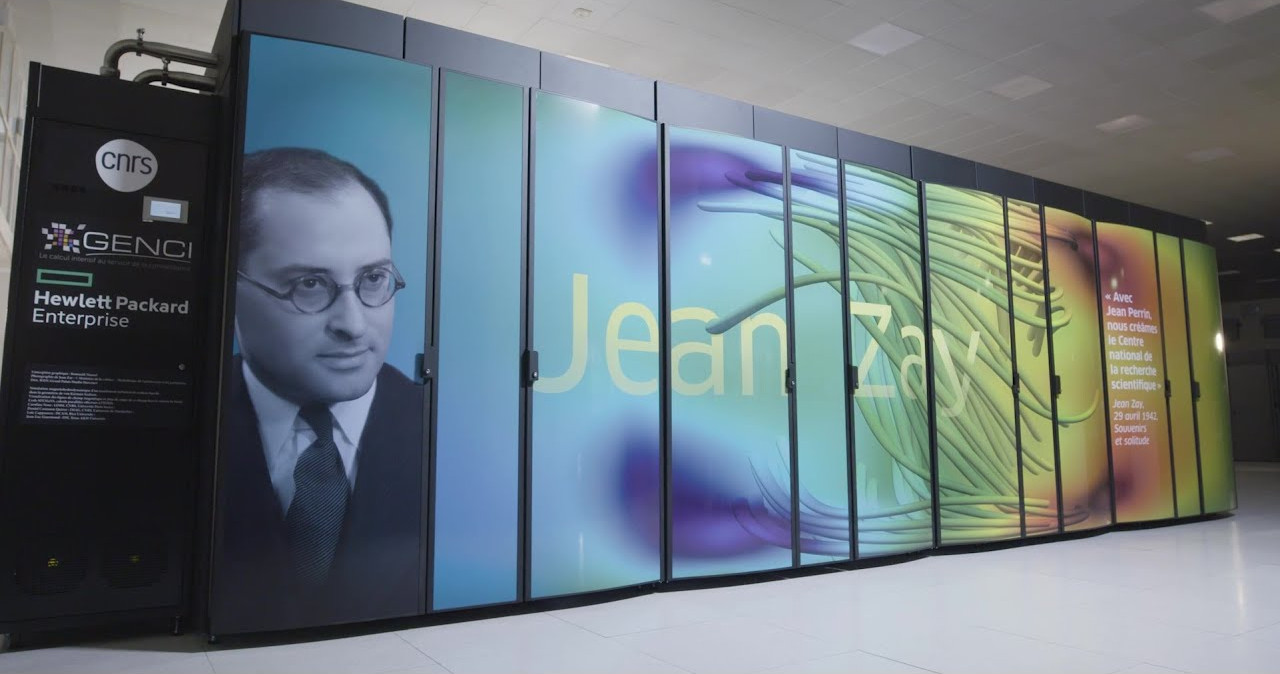
\includegraphics[width=0.7\linewidth]{pictures/Jean_Zay.jpg}
  \end{center}

  \begin{itemize}
    \item Nodes: 2$\times$ 20-cores \textsf{Intel Xeon Gold 6248 @ 2.5Ghz}, ``\emph{Cascade Lake}''
    \item Running time: 35 minutes on 512 nodes.
    \item Complete recovery using 512 consecutive output bytes.
    \end{itemize}
    
\end{frame}
%%% Local Variables:
%%% mode: latex
%%% TeX-master: "../main"
%%% End:
